\documentclass[letterpaper, 12pt, notitlepage]{report}
\usepackage[plainpages=false, colorlinks, urlcolor=black, citecolor=black,
	linkcolor=blue]{hyperref}
\usepackage{graphicx}
\usepackage[utf8]{inputenc}
\usepackage{txfonts}
\usepackage{listings}
\usepackage{multirow}
\usepackage[french, spanish, english]{babel}
\usepackage{epsfig}
%\usepackage[utf8]{inputenc}
\usepackage{sty/utfsm_tesis}
\usepackage{sty/xtocinc} %Include Table of Contents as the first entry in TOC
%\usepackage[dvips]{epsfig}
%\usepackage{psfig}

%% Margenes segun Normas
%% Ancho Legal 21,59cm /  8,5in
%% Alto  Legal 33,02cm / 13,0in
%\paperheight    27.81cm % alto letter
%\paperwidth     21.59cm % ancho
%\hoffset        -1.0in % Seteo a 0 el margen izquierdo
%\voffset        -1.0in % Seteo a 0 el margen superior
%\oddsidemargin  3.80cm % Margen izquierdo (pag. impar)
%% \evensidemargin 2.55cm % Margen izquierdo (pag. par) Acrobat Winkk
%\evensidemargin 2.59cm % Margen izquierdo (pag. par)
%\topmargin      1.00cm % Margen superior
%\headheight     5.00mm % Ancho encabezado
%\headsep        8.00mm % Separacion encabezado-cuerpo
%\textheight     23.5cm % Alto cuerpo
%\textwidth      15.2cm % Ancho cuerpo
%\footskip       1.30cm % Separacion piepag-cuerpo
\parindent      0em
\parskip        2ex

% Fuzz -------------------------------------------------------------------
\hfuzz2pt

% \oddsidemargin	 0cm	% Ancho Legal 21,59cm
% \evensidemargin 0.5cm	% Alto	Legal 35,56cm
% \textwidth	 16.5cm
% \topmargin	  -1.5cm
% \textheight	 22cm

\newlength{\defbaselineskip}
\setlength{\defbaselineskip}{\baselineskip}

\newcommand{\setlinespacing}[1]%
	   {\setlength{\baselineskip}{#1 \defbaselineskip}}
\newcommand{\doublespacing}{\setlength{\baselineskip}%
			   {1.3 \defbaselineskip}}
\newcommand{\singlespacing}{\setlength{\baselineskip}{\defbaselineskip}}

\lstloadlanguages{C++, sh, IDL, make}
\lstset{basicstyle=\small\sffamily, commentstyle=\slshape,
        numbers=left, numberstyle=\tiny, numbersep=10pt,
        extendedchars, frame=lines,
        floatplacement=ht, captionpos=b,
        defaultdialect=[CORBA]IDL}

\ingciv

\copyrightyear{2009} \submitdate{Nov 2009}
\convocation{November}{2009}

\title{ACS Component Code Generation Framework}
\author{Nicol\'as Troncoso}

\newcommand{\doctitle}{ACS Component Code Generation Framework}

\begin{document}
\selectlanguage{english}


\profguia{Dr. Horst H. von Brand}
\profcorr{Sr. Jorge Ibsen}

%\begin{titlingpage}
\begin{center}
  \begin{tabular}{c}
    \hspace{0.2cm}
    \begin{tabular}{c}
        \LARGE{UNIVERSIDAD T\'ECNICA FEDERICO SANTA MAR\'IA}\\
        \LARGE{DEPARTAMENTO DE INFORM\'ATICA}\\
        \LARGE{VALPARA\'ISO -- CHILE}\\
        \hspace{8.0cm}
        %\vspace{1.2cm}
    \end{tabular}
    \hspace{0.2cm}
  \end{tabular}

  \begin{figure*}[h!]
  \begin{center}
  
\includegraphics[height=3cm]{images/utfsm}
  \end{center}
  %
\epsfig{file=images/utfsm.eps,height=3cm}
  \end{figure*}

  \vspace{2.0cm}

  \LARGE{\doctitle}

  \vspace{1.0cm}

  \LARGE{NICOL\'AS TRONCOSO CARR\`ERE}

  \Large{\href{mailto:ntroncos@inf.utfsm.cl}{ntroncos@inf.utfsm.cl}}

  \vspace{1.0cm}

  \LARGE{MEMORIA PARA OPTAR AL T\'ITULO DE\\
         INGENIERO CIVIL EN INFORM\'ATICA}

  \vspace{1.5cm}

  \normalsize{}

  \Large{PROFESOR GU\'IA:  HORST H. VON BRAND}

  %\vspace{0.3cm}

%  \vspace{0.5cm}

 % \textbf{PROFESOR CORREFERENTE:  }

  %\vspace{0.3cm}
\end{center}

\vfill \centering XXXXXX -- 2009

\end{titlingpage}

%%% Local Variables:
%%% mode: latex
%%% TeX-master: "../thesis"
%%% End:

%\thispagestyle{empty}
%\begin{titlingpage}
\begin{center}
  \begin{tabular}{c}
    \hspace{0.2cm}
    \begin{tabular}{c}
        \LARGE{UNIVERSIDAD T\'ECNICA FEDERICO SANTA MAR\'IA}\\
        \LARGE{DEPARTAMENTO DE INFORM\'ATICA}\\
        \LARGE{VALPARA\'ISO -- CHILE}\\
        \hspace{8.0cm}
        %\vspace{1.2cm}
    \end{tabular}
    \hspace{0.2cm}
  \end{tabular}

  \begin{figure*}[h!]
  \begin{center}
  
\includegraphics[height=3cm]{images/utfsm}
  \end{center}
  %
\epsfig{file=images/utfsm.eps,height=3cm}
  \end{figure*}

  \vspace{2.0cm}

  \LARGE{\doctitle}

  \vspace{1.0cm}

  \LARGE{NICOL\'AS TRONCOSO CARR\`ERE}

  \Large{\href{mailto:ntroncos@inf.utfsm.cl}{ntroncos@inf.utfsm.cl}}

  \vspace{1.0cm}

  \LARGE{MEMORIA PARA OPTAR AL T\'ITULO DE\\
         INGENIERO CIVIL EN INFORM\'ATICA}

  \vspace{1.5cm}

  \normalsize{}

  \textbf{PROFESOR GU\'IA:  HORST H. VON BRAND}

  %\vspace{0.3cm}

  \vspace{0.5cm}

  \textbf{PROFESOR CORREFERENTE:  }

  %\vspace{0.3cm}
\end{center}

\vfill \centering XXXXXX -- 2009

\end{titlingpage}

%%% Local Variables:
%%% mode: latex
%%% TeX-master: "../thesis"
%%% End:

%\thispagestyle{empty}
%\cleardoublepage
\vspace*{\fill}

%\emph{Acknowledgements \ldots}

\begin{center}
\emph{Gracias a todos los que hicieron posible este trabajo, resultado final de
un largo proceso que ha involucrado incontables personas y ense\~nanzas.}

\vspace{0.3cm}

\emph{En especial quiero agradecer a:}

\vspace{0.3cm}

\emph{Las personas que guiaron este trabajo y le dieron forma, desde su
origen:\\ Jorge Ibsen, Gianluca Chiozzi y  Horst H. von Brand.}

\vspace{0.3cm}
\emph{Matias Mora requiere una menci\'on especial ya que fue una de las
personas que me presion\'o hasta el cansancio para que probara el generador con un modelo
complejo, gracias a todo lo que hinch\'o es possible que me titule en esta fecha.}

\vspace{0.3cm}
\emph{Gracias a Bogdan, Victor y Matias quienes aportaron comentarios y revisiones
de este texto.}

\vspace{0.3cm}
\emph{Gracias a mi familia, quienes no perdieron la f\'e\\ y mis amigos.}

\vspace{0.3cm}
\emph{Gracias a ALMA-CONICYT proyecto 3106008, y a sus colaboradores.}
\end{center}

\vspace{0.3cm}
\hspace{11cm}
\emph{Nicol\'as}


\vspace*{\fill}


% \end{dedication}
%\thispagestyle{empty}
%\cleardoublepage

%%% Local Variables:
%%% mode: latex
%%% TeX-master: "../thesis"
%%% End:

%\bibliographystyle{alpha}
%\maketitle
%\frontmatter
%%\thispagestyle{empty}
%\vspace*{\fill}
%
%\selectlanguage{english}
%\begin{center}
%\begin{LARGE}\textbf{Abstract}\end{LARGE}
%\end{center}
\prefacesection{Abstract}
Model driven code generation to ease the use of a complex framework like ACS.
Code generation reduces the number of Lines Of Code (LOC) crafted by a developer,
hence the number of errors per LOC.
This approach also makes it easier for the newly introduced
to the framework to get a quicker grasp developing application.
The work done in the thesis details the specific of a code generator for the ACS framework,
introducing the
model driven development as a novel feature for the framework.
The generation framework presented in this work
is based on transforming an UML Model
into an actual implementation in the
ACS component/container framework.
The output of the generation process
is readily usable by the developer,
and further refinement and complexity may be introduced
from a working start point.
%\vfill

%%% Local Variables:
%%% mode: latex
%%% TeX-master: "../thesis"
%%% End:

%\selectlanguage{english}
%\newpage
%\theglossary
%\begin{table}[h!t]
  \begin{tabular}{ll}
    ACS   & ALMA Common Software \\
    ALMA  & Atacama Large Millimeter/submillimeter Array \\
    BACI  & Basic Control Interface\\
    CDB   & Configuration Data Base\\
    CONICYT & Comisi\'on Nacional de Investigación Cient\'ifica y Tecnol\'ogica\\
    CORBA &  Common Object Request Broker Architecture\\
    CSRG  & Computer Systems Research Group \\
    ESO   & European Southern Observatory \\
    ICD   & Interface Control Document\\
    IDL   & Interface Definition Language \\
    LOC   & Lines Of Code\\
    MARS  & Maintenance And Repair System\\
    NRAO  & National Radio Astronomy Observatory \\
    NTT   & New Technology Telescope\\
    OAW   & Open Architecture Ware\\
    OBV   & Object By Value\\
    OMG   & Object Management Group \\
    ORB   & Object Request Broker \\
    TAO   & The ACE ORB \\
    TCP   & Transmission Control Protocol \\
    UML   & Unified Modeling Language\\
    UTFSM & Unversidad T\'ecnica Federico Santa Mar\'\i a \\
    VLT   & Very Large Telescope\\
    WSF   & Workstation Software Framework\\
    XMI   & Extensible Markup Language Metadata Interchange\\
    XML   & Extensible Markup Language\\
    XSD   & Extensible Markup Language Schema Document\\
    XSLT  & Extensible Stylesheet Language Transformations\\

  \end{tabular}
\end{table}

%%% Local Variables:
%%% mode: latex
%%% TeX-master: "../thesis"
%%% End:

%\cleardoublepage
%\tableofcontents
%\cleardoublepage
%\listoffigures
%\cleardoublepage
%\listoftables
%\cleardoublepage
%\lstlistoflistings
%\cleardoublepage
%
%\mainmatter
%\cleardoublepage
\ack{include/acknowledgements}			   % Incluir Archivo con Agradecimientos
\resumenesp{include/abstractes}	      % Incluir Resumen
\resumening{include/abstract}		   % Incluir Abstract
\abreviaciones{include/glossary}   % Incluir Abreviaciones

\beforepreface
\afterpreface
%\numberwithin{equation}{chapter}
\chapter{Introduction}
\label{ch:introduction}

Chile has huge potential for astronomical observation,
because it is the home of the majority of the most important observatories
in the world,
and the favorite place for further projects planned
to be constructed during the next decade.
With the clearest skies in the world,
Chile is becoming an astronomical power.
Some of the already installed international observatories are
La Silla (NTT, ESO-3.6),
Paranal (VLT),
Cerro Pach\'on (Gemini, SOAR),
Cerro Tololo (Blanco),
and Las Campanas (Magellan).
They are mainly financed by European and North American public organizations.

In addition,
the currently largest astronomical project
is under construction on the Chajnantor plateau
in the Atacama desert:
The Atacama Large Millimeter/submillimeter Array (ALMA)~\cite{ALMA-WEB}.
This will be a radioastronomy observatory,
formed by at least 54 12-meter diameter antennas and
12 7-meter diameter antennas,
which will act together as one big interferometer.
ALMA is a partnership between Europe (ESO),
North America (NRAO), and Japan (NAOJ).
It is expected to be fully operational by late 2012.

As part of the cooperation with the Chilean government,
ALMA is funding scientific development at Chilean Universities
with around half a million dollars annually.
In this context,
the Computer Systems Research Group (CSRG)
at Universidad T\'ecnica Federico Santa Mar\'\i a
is collaborating since 2004 with the development of ALMA software.
This work is currently financed by the ALMA-CONICYT fund,
and is done in close coordination
with the ALMA ACS and Control subsystems development.

Besides the work for the ALMA project,
CSRG is also collaborating with the Chilean astronomy community in other ways.
Some work has been done together with astronomy departments
at some other Universities,
implementing parts of the ALMA software to be used in smaller optical telescopes.

The following description of ALMA software follows~\cite{avarias08:_DDS_vs_NS}.
ALMA software
is built on top of the ALMA Common Software (ACS)~%
 \cite{chiozzi01:_ACS,gianluca06:_ACS_overview}
infrastructure framework.
%This is a CORBA based framework that
%aims to be an extensible platform
%for astronomical and non astronomical projects.
%Having this in mind this document presents a review
%of the current status of code generation,
%it benefits, and its applicability in ACS.
The ACS framework consists of a collection of common
patterns, components, and services. The heart of ACS is an component model
based on Distributed Objects implemented as CORBA~\cite{CORBA-OMG02} objects.
ACS is based on experience accumulated with similar science projects in the
astronomical and particle accelerator contexts, reusing concepts and
technology used previously like VLT Common
Software~\cite{sivera01:_vlt_overview}. Although designed for ALMA, ACS can
and is being
used in other control systems and distributed software projects, since it
has been implemented to be a generic control framework using generic design
patterns and components off the shelf~%
\cite{chiozzi08:_enabling_softw_sharin}.
Through the use of standard constructs and components, non-ACS developers
can easily understand the architecture of software modules. This makes
maintenance affordable even on a very large software project like ALMA.


As part of the ALMA-CONICYT fund collaboration,
CSRG has already contributed to ALMA software in
various aspects, such as a study of real time capabilities~%
  \cite{araya08:_verifiying_ACS_RT_periodic_properties,%
       tobar09:_real_time_time_service_ACS}
, in the area of control software simulation framework~%
  \cite{mora08:_hardw_devic_simul_framew_alma_contr_subsy,%
        mora08:_towar_gener_hardw_devic_simul}
, developed a scheduling prototype algorithm~%
  \cite{saez09:_sched_protot_amateur_teles_contr_acs},
  a generic automatic pointing system~%
  \cite{staig08:_refer_implem_gener_autom_point_system},
  and an amateur telescope control system~%
  \cite{tobar08:_csat_gtcs, tobar08:_CSAT_final_status}
  a hardware end to end example~\cite{valencia07:_H3E} for
  the ACS framework,
  and studied the feasibility of DDS as a replacement for the notification
  channel~\cite{avarias08:_DDS_vs_NS}.

As part of this collaboration,
specifically through project ALMA-CONICYT~\#31060008,
the author presents an undergraduate
thesis to cover some novel aspects which require attention
but have not yet been developed by CSRG nor the ALMA computing group.

\section{Problem Approach}
\label{sec:problem-approach}
Modern software control systems
involve multiple subsystems
and devices.
Projects start with final designs to be implemented,
but during the development of the project
the designs are subject to redefinitions,
redesigns and changes.
As~\cite{farris07:_device_driver_code_gener_framew,%
         farris06:_generating_software_modules}
adequately state,
coding a large codebase requires an
army of programmers.
A better approach is to use model-driven programing,
where the code is generated automatically
by a generator, based on a model.
This directly impacts the error per line of code
(since it takes over many routine, error-prone tasks)
and helps enforcing a single coding style for
a large portion of the code base.
Benefits of such an approach are that
it makes it easier to accommodate model changes,
and
it improves productivity since developers
can focus on business logic
instead of details of implementation.
Besides the above benefits,
improvements in the generator translate directly
into improvements in the whole generated code base.

\section{Objectives}
\label{sec:objectives}
ACS (Alma Common Software) could do with more automatically generated code.
It should be possible to write software components that use the framework
in an easier way than its done today.
Having this in mind is that the author proposes a thesis that accomplishes:
\begin{enumerate}
\item
  Code generation starting from a model
  UML~\cite{UML-WEB}
  (and/or text representation). UML (Unified Modeling Language) is a
  software modeling specification maintained by the Object Management Group (OMG)~%
  \cite{OMG-WEB}
  \begin{enumerate}
     \item Create IDL~\cite{OMG-IDL} files. This implies creating a full implementation of the
     UML model as an IDL file so it may be compiled by IDL compilers.
     \item Create a base class implementation starting from a class diagram.
     Base classes will be functional as they implement the
     relevant interfaces of the ACS framework.
     \item Create CDB XML schemas. CDB is the Configuration Data Base, this database informs
     the framework about the available software components.
     The database checks the component against an XML schema that defines the software
     component properties.
     \item Define the type mapping between the UML model representation
     and the specific language implementation.
  \end{enumerate}
\item
  Integrate design patterns to the code during the generation process.
\item
  Generate code for one of the ACS supported languages;
  in particular, Java.
\item
  Finally,
  validate the proposed solution through external opinions,
  current experience,
  and generating example implementations of a variety of models
  through a prototype implementation.
\end{enumerate}

\section{Document Structure}
\label{sec:documentStructure}
The document is structured as follows:
In chapter~\ref{ch:technology-overview} a review of
available technologies is made,
presenting different code generator
frameworks upon which this thesis is based.
Section~\ref{sec:code-generation:ACS} talks about
the current status of code generation in ACS,
section~\ref{sec:code-generation:impact}
details benefits that this thesis proposes.
Chapter~\ref{ch:architecture} talks about the
architecture of the proposed solution.
Chapter~\ref{ch:verification} details the verification
of the proposed solution.
Section~\ref{sec:test-configuration} sets the
testing framework used for validation.
%Section~\ref{sec:results-comparisons} presents the results
%of the validations.
Finally chapter~\ref{ch:conclusions} shows the conclusions
and final remarks of this undergraduate thesis.

%%% Local Variables:
%%% mode: latex
%%% TeX-master: "../thesis"
%%% End:

\chapter[Technology Overview]{Technology Overview}
\label{ch:technology-overview}
This chapter glides over the current
code generator technologies
that are relevant in the ACS framework context.
The main scope of this thesis
is the generation of backend code,
for that reason only tools suited for this purpose
are discussed.

Program transformation has applications and uses
in many areas of software engineering,
including compilation,
optimization~\cite{grune02:_compiler_design},
refactoring,
program synthesis,
software renovation,
and reverse engineering~\cite{muller00:_rever_engin, RE-WEB}.
The aim of program transformation is to increase programmer productivity
by automating programing tasks,
thus enabling programing at a higher-level of abstraction,
and increasing maintainability and re-usability~\cite{visser01:_asurvey}.

Program transformation may be divided roughly into the areas of
translation and rephrasing.
A \emph{translation} involves transforming a program from a source language
into a ``different'' target language.
Examples of such transformations are compilers such as
GCC~\cite{GCC-WEB},
TAO IDL~\cite{TAO-WEB},
\mbox{OmniOrb} IDL~\cite{OMNIORB-WEB},
jacOrb IDL~\cite{JACORB-WEB}.
Others are model to code transformations,
like the
ACS Error definition system~\cite{jeram02:_ACS_error_system}.

\emph{Rephrasings} are transformations that take an input program
and produce an output in the same language.
Rephrasing tries to say the same thing using different words.
The main scenarios where this is used are optimization,
refactoring,
and renovation.

\section{Generic Program Transformation (Code Generation)}
\label{sec:translation}

The main focus of the survey in this section
is the assessment of translation technologies
for use in the ALMA project.
This case study is aimed at finding proper tools and methods
to transform high level program definitions
into a high level language implementation
as is done by TAO, OmniOrb and JacOrb when transforming IDL representations.
This survey covers generic tools and special purpose tools.
The objective is to review
different technologies.

\subsection{IDL Transformations}
\label{sec:IDL-transformations}
Interface definition language,
or IDL for short,
is a specification language used to describe a software component's interface.
This language is part of the CORBA specification~\cite{CORBA-WEB, OMG-IDL, CORBA-OMG02},
which makes it a commonly used standard,
in particular it is widely used in ACS since ACS is CORBA-based.
IDL is the language used to describe the
interfaces that client objects call and object implementations provide. An interface
definition written in IDL completely defines the interface and fully specifies
each operation’s parameters. An IDL interface provides the information needed
to develop clients that use the interface’s operations.
This description may then be used
to generate language specific implementations of such interfaces,
making it possible to call objects written in one language
from clients written in another in a transparent manner.
The following are implementation examples of IDL transformations,
in particular the ones in common use in ACS.
\begin{description}
\item[The ACE ORB (TAO)~\cite{TAO-WEB}:]
  A CORBA C++ Object Request Broker (ORB).
  This tool offers an IDL compiler that creates a C++ representation
  of the interface.
\item[omniORB~\cite{OMNIORB-WEB}:]
  A robust high performance CORBA ORB that
  offers an IDL compiler for C++ and Python.
\item[jacOrb~\cite{JACORB-WEB}:]
  A CORBA Java ORB that
  provides an IDL compiler for the Java language.
\end{description}
These are perfect examples of a program translator (code generator).

\subsection{Code Generation in VLT Software}
\label{sec:code-generation:VLT}
Very Large Telescope (VLT) Software~\cite{filipi99:_vlt_software}
is a common proprietary middleware platform
which provides common services such as messaging, persistence, error handling and logging.
It also provides several utility programs, some with graphical user interface, to make development and debugging
of VLT applications easier.
To ease the development of VLT applications a dedicated framework is used.
The Workstation Software Framework (WSF)~\cite{andolfato09:_wsf}
is a state machine model driven development
designed to generate applications based on ESO VLT software.
Where state machine models are used to generate executables.
The framework provides code generation and supports hierarchical state machines, generating readily usable code.

\subsection{ALMA Control Software: Hardware Device Code Generator}
\label{sec:control-generator}
ALMA Control software uses a model driven approach
to generate code that controls the underlying hardware~%
  \cite{farris06:_generating_software_modules}.
Information from the hardware ICD (Interface Control Document)
is captured in the form of spreadsheets (using Microsoft Excel 2003)
that contains detailed information about the device,
its monitor and control points,
and its data monitor points that are to be permanently archived.
The spreadsheets are saved as XML documents~%
  \cite{farris07:_device_driver_code_gener_framew}.
Such a XML document is later fed to a template based code generator
that produces code that runs seamlessly in the ACS framework.
The generator used is OAW (Open Architecture Ware)~%
  \cite{OAW-WEB}, a modular generator framework implemented in Java.
It supports parsing of arbitrary models,
and a language family to check and transform models
as well as to generate code based on them.

An important factor to consider in this code generator framework
is the automatic generation of a simulation environment~%
  \cite{mora08:_towar_gener_hardw_devic_simul}.
This enables developers to test their code as soon as possible
getting a minimum assurance that the new code works.

The shortcoming of this code generator
is that it is specific for ALMA Control Software,
and it is detached from the ACS software release cycle.
This means that extra modifications are required by the CONTROL
software team when a new ACS delivery includes changes in the framework.
Notwithstanding, the Control Software generator is in production
(it is considered to be delivered and complete)
and no new design enhancements are foreseen in the near future.
An enhancement beyond the scope of this undergraduate thesis
would be to integrate the control generator with the new
generator proposed by the author.

\section{Code Generation in ACS}
\label{sec:code-generation:ACS}
ALMA Common Software as a framework supports code generation to some extent.
CORBA stubs (see~\ref{sec:IDL-transformations})
and error definitions (see~\ref{sec:ACS-error-system})
for all languages supported by ACS are automatically generated.
Also,
ACS provides a state machine code generator
which to some extent makes ACS a generated code framework.
Having all the previous generation facilities,
the core programing is done in the software components.
Nevertheless,
writing software components is still a repetitive task,
the overhead is the same for all components~%
  \cite{grega05:_acs_comp_cont_fram_tut}.
To circumvent the overhead of repetitive tasks some
ACS code generators have been proposed, like
the ACSgenerator described in~\ref{sec:acs-generator}.

\subsection{ACS Error System Code Generator}
\label{sec:ACS-error-system}
The ACS Error System~\cite{jeram02:_ACS_error_system}
is based on XML (Extensible Markup Language)
and XSLT (Extensible Stylesheet Language Transformations)~%
 \cite{XSLT-WEB} code generation.
Types and their corresponding codes are defined in XML files
in an ACS language independent way.
Which will in turn be converted to the specific
Java,
C++ and
Python implementation.
For each error definition type,
a unique XML file must be written by the developer.
This file is used by the XSLT transformation to produce the code.
The generated code contains a set of completion and exception helper classes,
one for each error code.
There is a separate XSLT for each programming language
and one specifically for IDL.
Currently all code generation is done automatically
during system build
by using a target in the ACS \lstinline[language=sh]!Makefile!.
This code generator is considered to be complete,
at this time it is being used in production
in ALMA software.

\subsection{ACSGenerator}
\label{sec:acs-generator}
ACSgenerator is a community code contribution to the ACS project.
It is based on bdsGenerator~\cite{ACS-CONT}
which was created to use ACS sofwate
with the Hexapod Telescope~\cite{HPT-WEB}.
The bdsGenerator system is a C++ hardcoded template based code generator
that parses IDL files and creates
a C++ ACS component module.
ACSgenerator further extends the bdsGenerator work
providing very advanced code generation.
At this time ACSgenerator
only creates C++
component modules making it
complementary to the work in this thesis.
The work proposed in this thesis aims
at solving some limitations of ACSgenerator,
such as
one interface per module,
and simple template extension.
The expirience of this generator should be used
when extending the ACS generator to the C++ implementation
in an effort to merge the functionality of both.

\section{Impact of Code Generation}
\label{sec:code-generation:impact}
During the past decade
there has been an
upsurge in the use of code generators
in an attempt to deliver enterprise
software to the market as
quickly as possible~\cite{ACG}.
Even though
automated code generation is not a new concept,
it had received
relatively little recognition.

Expertise is an intangible but unquestionably valuable commodity.
People acquire it slowly,
it takes a long time for a novice to become an expert.
Design patterns~\cite{gamma94:_design_patterns}
are a way to capture expert knowledge
and convey it to novice developers.
The drawback with this approach is that a design pattern
is only know-how and not an implementation per se.
Budinsky et al. describe an automatic code generator~%
   \cite{budinsky96:_automatic_code_generation}
which addresses this issue by generating code
using a specified design pattern.
This approach ensures consistency throughout the development.

Support of software evolution and maintenance is at hand
when generating code from a formal definition language.
Such a definition may be appropriately translated
to cope with underlying platform changes
without major developer interaction~\cite{floch95:_automatic_code_generator}.
A framework change is possible without cumbersome refactoring
of all the software built on top of the framework,
since the change can be made in the generator.

Some of the mayor concerns at hand
when working with code generation
is
keeping the generated code
clean and humanly readable.
This is important for this project since
the way defined by ALMA software development
to handle problems in generated code
is to debug
the generated code,
manually
tweaking it until the problem is found and fixed,
and the fix is then introduced into the generation process.
This debug process can be extremely complex if the
generated code is not well structured.
Another important pitfall of the code generation
is that if a bug is introduced in the generated code
this bug will be present all over the generated software.
At the same time, since the generation process is common,
fixing a bug
fixes it in all the generated software.
On the other hand,
if the generator itself is opaque,
there will be a tendency to fix the generated code instead of the generator.
These issues should be kept in mind when
working with code generation.

%%% Local Variables:
%%% mode: latex
%%% TeX-master: "../thesis"
%%% End:

\chapter{Architecture of the Solution}
\label{ch:architecture}
Following the industry standard and a requirement from
the ACS software group,
UML (Unified Modelling Language)~\cite{UML-WEB} was chosen as the model definition language.
As ACS ships with Open Architecture Ware (OAW)~\cite{OAW-WEB}, it was natural to use
this tool to build the ACS code generator
since it avoids introducing new external
software into the ACS framework.

The greatest challenge to achieve a proper code generation for the ACS framework
was to properly translate an UML model into generated code.
The overall architecture proposes to start from
an UML model in XMI 2.0 UML~\cite{OMG-WEB} format,
and use Open Architecture Ware to transform this model into an actual implementation.
The generated implementation consists in
the Java component code,
the corresponding IDL interface,
an XSD Schema file
and
an example configuration database usable for immediate testing.
The generated Java component is a ready component
in the sense that it may be instantiated
by the ACS component without need of extension by the developer.
This provides and easy and first verification that the generated code is working properly.

The general architecture of this code generator
allows the developer to generate ACS
components and
characteristic components.
The former are the simplest case and the later add
additional complexity when generating code
since they require access to the BACI interface.
BACI, the Basic Control Interface
is a general purpose control framework.
It does not specify any specific control system,
but it restrict the space of definable objects
within a specific design and guidelines defined
in the BACI interface~\cite{plesko05:_baci}.
It is not required to have components and characteristic components
in different models.
The ACS framework is container/component based.
Hence ACS components are the basic
functional software element that can be created.
In case the control interface is needed
it is possible to define characteristic components
instead of simple components,
this will give the software implementation
access to BACI.
The ACS code generator
expects that classes identify their
behavior, either as components or as characteristic components,
using stereotypes and thus instructing the
code generation on how to proceed.

The generation flow will take the UML model as input and generate
the IDL interface, Java base code,
and a test CDB (ACS Configuration DataBase).
In the case of a class that is a
characteristic component,
a XSD (Extensible Markup Language Schema Document)
schema is generated as well.

\section{UML Model Specification}
\label{sec:uml-model-specification}
The UML model must comply with some specific stereotypes not specified in the UML standard
but relevant in the ACS framework. These stereotypes are enumerated in table~\ref{tb:stereotypes}.
\begin{table}
\centering
\begin{tabular}{|l|l|}
\hline \textbf{Stereotype} & \textbf{Description} \\
\hline \multicolumn{2}{|l|}{\textbf{Class Stereotype}} \\
\hline \texttt{<<CharacteristicComponent>>} & Indicates if the component is characteristic.\\
\hline \texttt{<<NOGenerated>>} & Indicates that this class must not be generated.\\
\hline \texttt{<<IDLStruct>>} & Indicates that this class must be treated as an IDL struct.\\
\hline \multicolumn{2}{|l|}{\textbf{Type Member Stereotype}} \\
\hline \texttt{<<ReadOnlyProperty>>} & The type uses the read-only BACI interface for properties.\\
\texttt{<<ReadWriteProperty>>} & The type uses the read/write BACI interface for properties.\\
\hline \multicolumn{2}{|l|}{\textbf{Function Member Stereotype}} \\
\hline \texttt{<<Asynchronous>>} & The method is implemented as an asynchronous method.\\
\hline
\end{tabular}
\caption{Stereotypes}
\label{tb:stereotypes}
\end{table}
Additionally,
it should be possible to specify data types which are not defined by the UML specification,
for example the \lstinline[language=IDL]!Sequence! data type. This type is declared and used extensively in the ACS framework.
If this non-standard data type is used in the model it should be used automatically in the generated code without
any special intervention.
Additionally the UML package name will be used by the code generator to name the \lstinline[language=sh]!jar! file, and the directory structure.
An important feature in the generation process is to define some class as
\texttt{<<NOGenerated>>}, this instructs the code generator
not to generate any implementation for it.
This is significant when doing complex extensions,
were it is possible that the developer does not want to generate code for a particular class,
but wants to keep the model complete so the generator may define extending classes
appropriately.

\section{Infrastructure}
\label{sec:infrastructure}
Along with the generated code,
the ACS module infrastructure is created as well.
This infrastructure is needed to properly compile and install and
ACS component,
independent of its implementation language.
This infrastructure is divided in various sub-directories
which contain essential information divided in different categories.
\begin{quote}
  \begin{description}
  \item[idl:] This directory contains the IDL interfaces and the XML
    definitions of the errors.
  \item[include:] This directory contains files with definitions,
    normally C++ header files.
  \item[src:] This directory contains the actual code and the ACS
    \lstinline[language=sh]!Makefile!.
  \item[config:] This directory contains the ACS schema specification
    if one is required.
  \item[doc:] This directory contains any additional documentation.
  \end{description}
\end{quote}
The directory structure is created automatically during the generation process.

\section{Non Generated Code}
\label{sec:non-generated-code}
It is not possible to fully generate the logic within the software component.
To achieve the full functionality of the component the developer must extend the generated code.
This scheme has been shown to work in the ALMA CONTROL software code generation~%
\cite{farris07:_device_driver_code_gener_framew,%
      farris06:_generating_software_modules}
where the generated code is extended by class inheritance.
The same approach is used in the ACS Code Generator,
a minimal working component is automatically generated,
but the internal logic must be added by the developer by means of class extension.

\begin{figure}[htp]
  \begin{center}
  \includegraphics[width=\textwidth]{images/generation}
  \end{center}
  \caption{Code Separation}
  \label{fg:generation}
\end{figure}

The main benefit of this approach is that it isolates
the generated code from the user written code.
The side effect of this is that code may be regenerated
multiple times without affecting user implemented code.
This is known as a code separation pattern as
seen in figure~\ref{fg:generation}.

During the development cycle
the base (generated) classes are created,
then the developer extends these classes
and implements complex functionality within the extensions.
This approach is used with the generated IDL
and generated Java files.
It is also possible to use the same
approach with the generated XSD files.

OAW provides a way to tell the generator which
parts it must generate,
by allowing the developer to delimit certain
regions of code as protected.
The code separation scheme described above was preferred over
region delimitation since the later
adds complexity to the generator
and
to the generated files themselves.

\section{Deployment Configuration}
\label{sec:deployment-generation}
The CDB is the database that holds the deployment configuration for ACS components.
It is not possible to deploy an ACS software module without it.
The code generator presented in this document generates a basic test CDB.
This CDB contains the Manager and components definition.
Every component (characteristic and non-characteristic) defined in the UML model is
inserted into the generated CDB. Thus, once code generation is done, the developer has
a ready to go test CDB with which he may readily instantiate the ACS components.

An additional feature which was specified as a requirement for this code generator
is the creation of a schema file when dealing with characteristic components. So, in addition
of creating the proper CDB files, the generator creates the schema file that validates the
CDB.


\section{Generation Workflow}
\label{sec:generation-workflow}
This section describes the steps taken
in order to convert an UML model into an
ACS system,
see figure~\ref{fg:generalWorkflow} for a general layout
of the steps to accomplish
the end to end generation task.
\begin{figure}[htp]
  \begin{center}
  \includegraphics[width=5cm]{images/general-workflow}
  \end{center}
  \caption{General Generation Workflow}
  \label{fg:generalWorkflow}
% Fixme: Place "IDL tasks", etc in an external column?
\end{figure}

Figure~\ref{fg:processWorkflow} shows the internal steps taken by the code generation.
The targets described in table~\ref{tb:oawtasks} are
tasks taken by the ACS code generator in order to generate
the ACS software module.
\begin{table}[htp]
\centering
\begin{tabular}{|l|l|}
\hline \textbf{Task Name} & \textbf{Description} \\
\hline \multicolumn{2}{|l|}{\textbf{IDL tasks}} \\
\hline \texttt{genidlCommon} & Generate common IDL files. Contains structs and enumerated types.\\
\hline \texttt{genidl} & Generate IDL files for every ACS component.\\
\hline \multicolumn{2}{|l|}{\textbf{Java Tasks}} \\
\hline \texttt{genjava} & Generate Java Helper and Java Base classes.\\
\hline \multicolumn{2}{|l|}{\textbf{ACS module tasks}} \\
\hline \texttt{genschema} & Generate Schemas in case of ACS characteristic component.\\
\hline \texttt{gencdb} & Generate test CDB.\\
\hline \texttt{genmake} & Generate Makefile.\\
\hline
\end{tabular}
\caption{OAW Tasks}
\label{tb:oawtasks}
% Fixme: Place "IDL tasks", etc in an external column?
\end{table}

The tasks described in table~\ref{tb:oawtasks}
show the different OAW targets
which are processed
in order to
generate an ACS software module.
Every task in independent of the
others, so
they may be interchanged, eliminated or
new steps could be added.
\begin{figure}[htp]
  \begin{center}
  \includegraphics[width=10cm]{images/oaw-workflow}
  \end{center}
  \caption{Generation Process Workflow}
  \label{fg:processWorkflow}
\end{figure}


\section{Extension and Modification of the Code Generator}
\label{sec:extension-modification}
As described before it is possible to
extend or modify the templates.
This can be done without big
invasions of the existing templates,
since custom templates may be defined
and their location
configured
in the \lstinline[language=sh]!workflow.oaw! file
under the targets described in table~\ref{tb:oawtasks}.
The same way alternate templates
are configured,
additional targets can
be added
to \lstinline[language=sh]!workflow.oaw!,
since as described before the
code generation targets are independent of each other.
This modularized approach was taken to enable extension and
to keep generation modules small and maintainable.

Extending or designing new templates
requires some expertise and knowledge of
the Xpand2 and Xtend languages,
yet the implemented templates
may be used as a staring point or tutorial
on how Xpand2 works.
OAW documentation clear, good, abundant and freely available,
and OAW has recently been merged with the
Eclipse Modeling Project~\cite{EMF-WEB},
widening its community support.

\section{Final Proposal}
\label{sec:final-proposal}
This section describes the final proposal for the ACS code generator.
This proposal takes into account
all the previous discussion,
further validation may be seen in chapter~\ref{ch:verification}.

\subsection{OAW Generation Process Specifics}
\label{sec:oaw-specifics}
OAW (Open Architecture Ware)~%
\cite{OAW-WEB} is a modular generator framework implemented in Java.
It supports parsing of arbitrary models,
and a language family to check and transform models
as well as generate code based on them.
It provides the following facilities:
Xtext, Check, Xpand2 and Xtend.
The architecture of the ACS code generator
is based on the later two.
Xpand2 provides a template base generation,
and Xtend provided a set of helper functions
to keep the templates clean.

The tasks that OAW executes are defined in the
workflow configuration (\lstinline[language=sh]!workflow.oaw! file).
This is an XML file which configures how
the model is parsed and which templates
should be applied to the model.

\begin{itemize}
  \item{\textbf{Parsing and navigating the model.}}
  OAW provides the flexibility to define
  in house model representations,
  as seen in the case of ALMA CONTROL Software~\cite{farris06:_generating_software_modules},
  or use factory shipped model parsers.
  In the specific case of the ACS code generator,
  since UML models are used,
  it is possible to use the UML model parser provided
  by OAW.
  The model representation is easily navigated
  since it is presented as an hierarchical structure,
  in the form of a series of containers related to other,
  where it is possible to ask for
  attributes, contained elements, or parent elements.
  The ACS code generator is designed to
  understand class diagrams.
  Having this in mind its possible to retrieve all
  the classes in the model as a list.
  Then it is possible to go in depth in each one of this
  class elements retrieving attributes, stereotypes, operations
  and relations to other classes.
  Then again for each class sub-element it is possible
  to retrieve their sub-elements, so on and so forth
  until leaf elements are reached.

  \item{\textbf{Applying the templates.}}
  The OAW Xpand2 templates are defined as
  dynamically replacing text.
  This is done by defining routines that
  fetch the required attributes from the parsed
  model and
  replace it in a text template.
  It is possible to define multiple output text files
  as well as a single output file
  in a single template file.
  This allows the generator to generate one file
  per class, and
  a single file for common class interfaces (IDLs).
  The text which is replaced in the template
  is embraced within the special characters
  \textbf{\flqq~~\frqq} (called guillemets).
  The replacement text may be a call
  to a function in Xtend or even an external Java
  call in case very complex substitutions are needed.
  This flexibility allows the template to be very small,
  but generate substantial files, or even multiple files,
  keeping the complexity of the template as low as possible.
\end{itemize}

\subsection{Design}
\label{sec:design}
The integrated design of the generator may be seen in figure~\ref{fg:design}.
The overall design is based on translating an UML model in XMI format
into an ACS Component.
This is done using:
\begin{enumerate}
    \item\textbf{OAW Workflow definition:}
    This defines the steps to be taken to generate the ACS component.
    In the case of this specific generator
    the steps defined in the workflow are the ones
    described previously in table~\ref{tb:oawtasks}
    \item\textbf{Template definition:}
    Each one of the defined tasks requires a separate template that will
    translate into a file. Each template is domain specific, so there must be one for each transformation
    that must be done (i.e., Java files, CDB files, etc).
    The input information for these transformations
    is the UML model that has been previously parsed by OAW.
    \item\textbf{Extension definition:} These are meant to be helpers to the \textbf{Template definitions}.
    They gather common transformation that are shared by all the domains. In the specific case
    of this generator they gather functions to detect if a class should be generated or not,
    and in what way it should, if it is an IDL
    \lstinline[language=IDL]!Struct!,
    \lstinline[language=IDL]!Component!,
    or \lstinline[language=IDL]!CharacteristicComponent!.
\end{enumerate}

\begin{figure}
  \begin{center}
  \includegraphics[width=\textwidth]{images/design}
  \end{center}
  \caption{Generator Design}
  \label{fg:design}
\end{figure}

All generated files are output to a directory defined in the OAW workflow file.
This directory is created so as to mimic an ACS template.
For this reason,
once the files are generated its possible to compile and install right away.

\subsubsection{Challenges Encountered}
This section describes the specific problem and challenges that were encountered
when developing the ACS code generator.
\begin{itemize}
  \item{\textbf{The templates get cluttered.}}
  The templates get cluttered very fast with tasks
  and
  statements that must be repeated.
  To solve this, the repetitive task or
  similar tasks were transferred to an
  extension file.
  This extension file is written in a
  functional language that OAW provides.
  Extension may be included in any template
  and help to keep the template simple.
  \item{\textbf{Mapping of types from UML to code is not direct.}}
  UML defines native type with caps for the first letter.
  For example,
  IDL does not support the type \lstinline[language=Java]!int!,
  and JacOrb translates a
  \lstinline[language=IDL]!long! into an \lstinline[language=Java]!int!,
  this created many type
  mismatches. To solve this problem
  special methods where implemented in the extension file.
  The methods translate an UML type into an IDL or Java type
  as required.
  \item{\textbf{Return types and return values for the Java code are not correct.}}
  This problem is similar to the one described in the previous item.
  The issue is that the Java code must return the type and value defined in IDL,
  which led to mismatches. The solution was to implement a method that gets the proper
  return type and value for the Java code. This method is also part of the
  extensions file.
  \item{\textbf{Definition of IDL structs and enumerated types lead to type redefinitions.}}
  To address this issue, OAW tasks \lstinline[language=sh]!genidl! (described in table~\ref{tb:oawtasks})
  was internally split into two steps.
  \begin{enumerate}
    \item Generate IDL structs and enumerated types into a common file.
    \item Generate other IDL files and include the common file.
  \end{enumerate}
  This also provides a more granular control
  when importing this IDL files from client code
  or external software module.
  \item{\textbf{Generation does not guarantee the order of IDL entities}}.
  This problem appears when using more complex models. If the XMI description
  is not ordered in a dependency sense, then the generated IDL code
  does not build since it uses structures that have not been defined yet.
  Dependencies within classes may be solved by forward declaration, but
  dependencies within IDL structs may not.
  Therefore the XMI file must be dependency ordered\footnote{%
  An experimental ordering function is being tested to circumvent this issue.
  This function should be ready for the release of the second prototype.}.
\end{itemize}


%%% Local Variables:
%%% mode: latex
%%% TeX-master: "../thesis"
%%% End:

\chapter{Verification}
\label{ch:verification}
This chapter presents a validation of the design proposed in chapter~\ref{ch:architecture}.
Section~\ref{sec:test-configuration}
presents the configuration used to perform the
validation tests.
Section~\ref{sec:external-review} presents one of the most important
aspect of the validation process,
the peer review
which was more than relevant to properly assess the status of this
work, and to identify promising lines of future work,
as mentioned in chapter~\ref{ch:conclusions}.
% Finally,
% section~\ref{sec:results-comparisons}
% presents additional results and comparisons with other work.

\section{Test Configuration}
\label{sec:test-configuration}
For testing purposes two models were generated,
these models cover the full spectrum of code that can be generated by
this work.
Both models cover a basic component,
and more complicated structures as enumerated in table~\ref{tb:stereotypes}.

At the time when implementation was begun,
the setup chosen was:
\begin{itemize}
\item\textbf{Operating System}: A virtual machine with Red Hat Enterprise Linux 4.4 (interchangeable with Scientific Linux 4.4).
\item\textbf{ACS}: ACS version 8.0.0 Back port Red Hat 4.4.
\item\textbf{OAW}: Version 4.1.3 with the itemis distribution.
\item\textbf{Modeling Tool}: Magic Draw 16.5
\end{itemize}

The models used are specified in figures~%
\ref{fg:MARSclassDiagram},~%
\ref{fg:ExtendedMARSclassDiagram} and~%
\ref{fg:BACIClassDiagram}.
The MARS model~\ref{fg:MARSclassDiagram} makes full usage of support of enumerated types
and \texttt{<<IDLStructs>>}.
The BACI Example is intended to test the generation of a characteristic component
including \lstinline[language=IDL]!readWrite! and \lstinline[language=IDL]!readOnly! characteristics.

\begin{figure}
  \begin{center}
  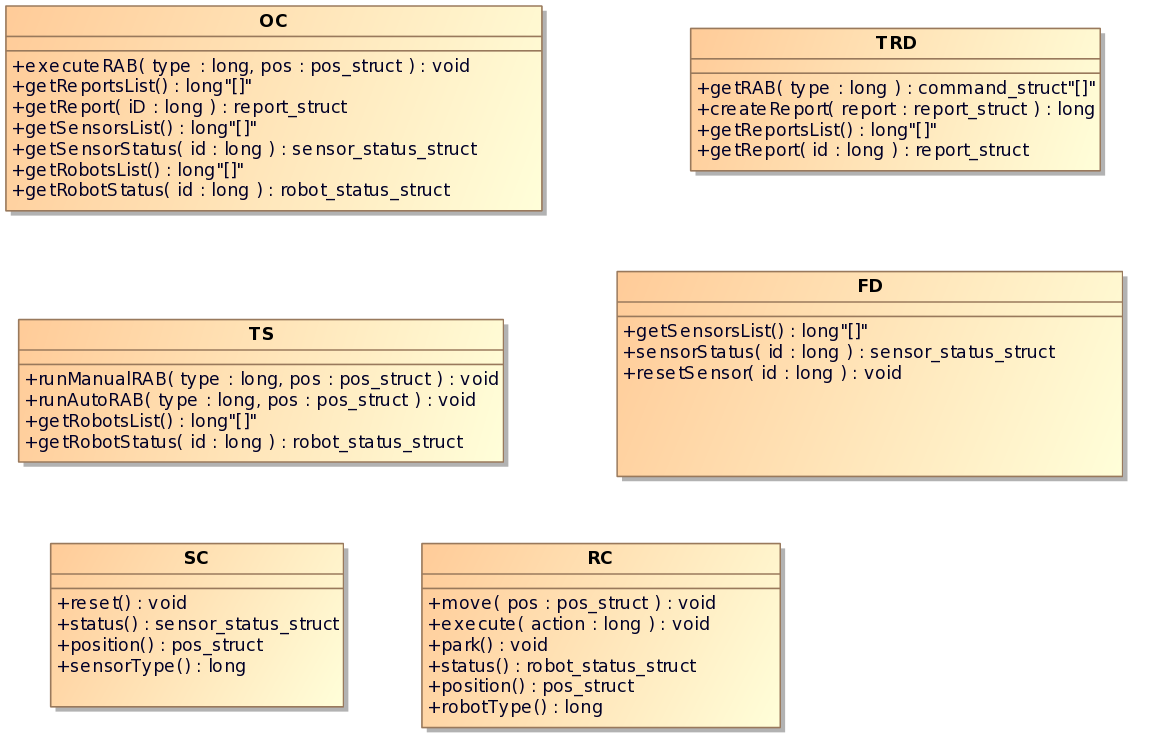
\includegraphics[width=\textwidth]{images/MARS-classdiagram.png}
% Fixme: Has grid lines in the background, text is too small to read
  \end{center}
  \caption{MARS Example Class Diagram}
  \label{fg:MARSclassDiagram}
\end{figure}


\begin{figure}
  \begin{center}
  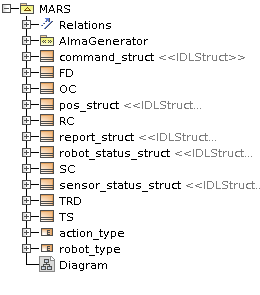
\includegraphics[width=0.65\textwidth]{images/MARS-classdiagram-full.png}
% Fixme: Completely unreadable, way too small
  \end{center}
  \caption{Extended MARS Example Class Diagram}
  \label{fg:ExtendedMARSclassDiagram}
\end{figure}

\begin{figure}
  \begin{center}
  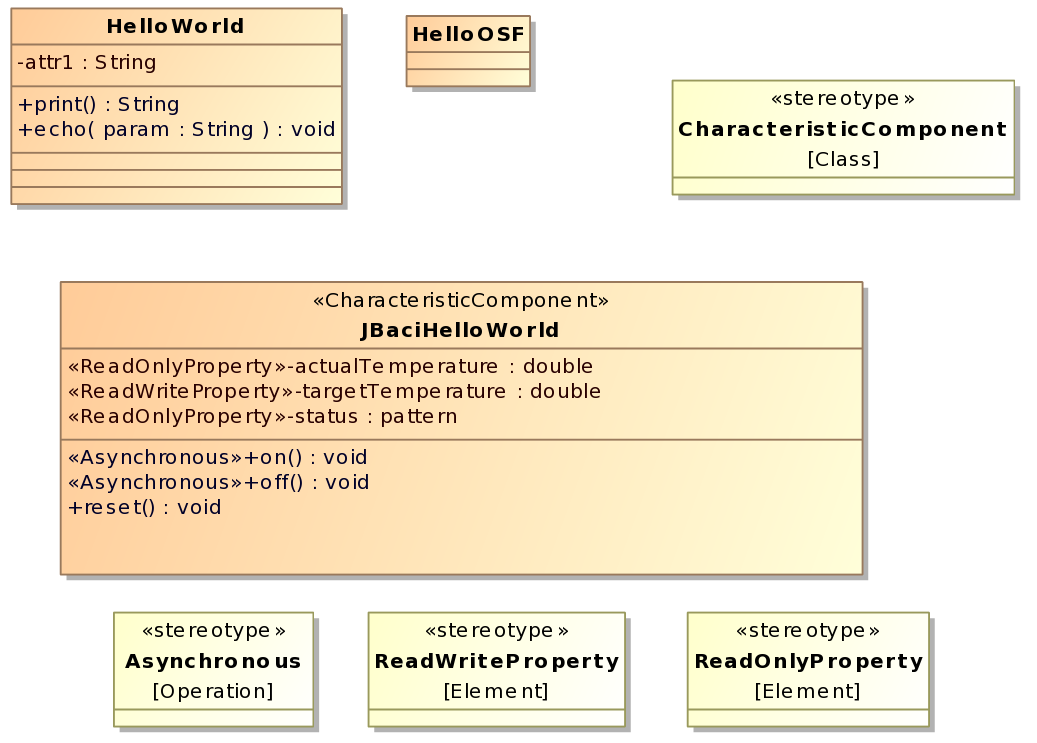
\includegraphics[width=\textwidth]{images/example-classdiagram.png}
  \end{center}
  \caption{BACI Example Class Diagram}
% Fixme: Completely unreadable, way too small
  \label{fg:BACIClassDiagram}
\end{figure}

After executing the ACS code generator as described by the workflow in
section~\ref{sec:generation-workflow},
the output files were tested initially by compiling and installing
the new software module.
Compilation is achieved using the generated \lstinline[language=sh]!Makefile!.
A strict requisite is that the generated code must
compile correctly and it should be possible to instantiate all classes.
This is manually checked during the verification process,
a test suite should be generated to automate this process.

\section{External and Peer Review}
\label{sec:external-review}
This work was followed closely by Gianluca Chiozzi,
Head of Software Instrumentation at ESO,
who had the opportunity to test preliminary versions of
the ACS code generator.
His comments and suggestions are gratefully acknowledged.
He presented a poster~\cite{chiozzi09:_acs_status} at
ICALEPCS 2009, where this generator is mentioned as
a future feature for ACS.

This work was also presented in the Advanced Track of
the 6th ACS Workshop,
which took place at UTFSM, on November $13^{th}-19^{th}$ 2009.
Positive feedback was received during
the presentations, including requests for new features which
should be addressed as future work (see section~\ref{sec:future-work}).

The MARS model (figure~\ref{fg:MARSclassDiagram}) was originally
designed for the
basic tutorial track of the 6th ACS Workshop,
but it evolved into a validation
suite for this project.
A portion of the generated code, specifically the IDL files,
was used during the basic track and a software implementation
of these IDL files
was implemented using the ACS framework.

%\section{Results and Comparisons}
%\label{sec:results-comparisons}
% As the title says results and comparison.
% Good comparison are Control Code generator
% ACS generator and state machine Generator.



%%% Local Variables:
%%% mode: latex
%%% TeX-master: "../thesis"
%%% End:

\chapter{Conclusions}
\label{ch:conclusions}
This work has produced a design and a
working implementation of a Model Driven
generator for the ACS framework.
The development process was based on an iterative process with hands on
experience and real examples that made shortcomings and modifications needed
in the design evident.
The shortcomings detected were addressed in the evolution to the actual implementation,
achieving a maturity such that the generated IDL files were
used for the 6th ACS Workshop Basic Track Live Example (see section~%
\ref{sec:external-review}).

The most remarkable features of the generation framework are:
\begin{itemize}
    \item The generated module is ready for compilation and usage as generated.
    No further development is required for initial testing.
    \item A pluggable module design was achieved, in the sense that adding
    an additional implementation language does not disrupt, nor cause great
    impact in the generation framework.
    \item The version of OAW used during development is the same as
    the one shipped by ACS-8.1. No porting efforts are required for integration.
\end{itemize}

The work of this undergraduate thesis complies
with the objectives defined in
section~\ref{sec:objectives} as follows:
\begin{enumerate}
\item
  \textbf{Code generation starting from a model
  (and/or text representation).}
  The input for the generation process is an UML model in the
  XMI (UML\,2.0) format.
  \begin{enumerate}
     \item \textbf{Create IDL files. This implies creating a full implementation of the
     UML model as an IDL file so it may be compiled by IDL compilers.}
     A full IDL implementation of the model is generated.
     This includes IDL structs and enumerated types, entities which were not
     considered in the preliminary design, but found to be essential during development.
     \item \textbf{Create base class implementation starting from a class diagram.
     This base classes will be functional as they will implement the
     relevant interfaces of the ACS framework.}
     Basic base class implementation is achieved, these base classes
     also have empty implementation of the complete interface defined by the IDL file.
     \item \textbf{Create CDB schemas. CDB is the Configuration Data Base, this database informs
     the framework about the available software components.
     The database checks the component against an XML schema that defines the software
     component properties.}
     CDB schemas are created where they are needed (ACS Characteristic Component).
     As an addition it was found necessary to create a test deployment CDB.
     This CDB is ready for use, and requires no developer intervention to be used as is.
     Doing this allows the developer to readily test the generated component,
     without spending time on the time consuming labor of defining a CDB.
     \item \textbf{Define the type mapping between the UML model representation
     and the specific language implementation.}
     This is internal to the code generator templates.
     Mappings to convert UML types to IDL and Java types
     are defined by extension methods.
  \end{enumerate}
\item
  \textbf{Integrate design patterns to the code during the generation process.}
  By using the code separation pattern the generated code is isolated from
  the developer implemented code. This allows the generator to use and insert
  patterns and abstraction levels without major impact on the hand-written code.
\item
  \textbf{Generate code for one of the ACS supported languages;
  in particular, Java.}
  Full support for Java components and Java Characteristic components was implemented.
\item
  \textbf{Validate the proposed solution through external opinions,
  current experience,
  and prototype implementation.}
  This objective has been achieved as described in chapter~\ref{ch:verification}.
\end{enumerate}

\section{Future Work}
\label{sec:future-work}
This work is an initial prototype
that provides a good base for a full featured
code generator for the ACS framework.
To achieve full featured status,
further work on this generator should implement
the following features and enhancements:
\begin{itemize}
   \item Support for C++ and Python ACS component implementations,
     and perhaps languages to be added in the future.
     Use the experience with other generators,
     like
     the ACSGenerator and the bdsGenerator,
     as a guide for this task.
   \item It should be possible to define the resources
   an ACS component will need during design, this way it would
   be possible to check usage at compile time, and ensure proper
   acquire and release cycle of such resources.
   \item Move common operation logic from manually implemented
   modules into the generated code.
   \item Identify common code chunks or repetitive chunks,
   and move them from the templates into their classes.
   They should be integrated using
   the \texttt{<<uses>>} code pattern.
   \item Flexible package definition, in the sense that it should be
   possible to define in the model
   the way the software modules should be grouped
   into packages, libraries and modules.
   \item Inheritance support between generated and non-generated code.
   This is required to provide support for more complex models.
   \item Provide exceptions support, in the sense that the model and
   generated file should make use of them, and the XML definition
   should be generated so ACS may use the ACS Error Generator to create
   the Exception definitions for all used languages.
   \item Provide an ACS model profile so the model definition does not
   have to rely on stereotypes.
   Currently it uses the type defined in the profile directly,
   that way new components and new characteristic components directly
   extend the ACS component and ACS characteristic component.
   \item Integrate the code generator into the ACS module workflow.
   This should define how code is generated, whether outside the ACS modules
   or inside the same ACS module. How are \lstinline[language=sh]!Makefile!s handled in the later case?
   \item Provide full model checking using an XSD or the OAW check facility.
   The model should be validated by the generator in the sense
   that it should guarantee that it can generate a sensible
   output from it. This is done in the ALMA Control Software,
   which might be used as a starting experience.
    \item Study the feasibility of integrating this work with the
    ALMA control software hardware device code generator
    described in section~\ref{sec:control-generator}.
\end{itemize}

%%% Local Variables:
%%% mode: latex
%%% TeX-master: "../thesis"
%%% End:


%\backmatter
%\cleardoublepage

\singlespacing
\cleardoublepage
\bibliographystyle{plain}

\bibliography{csrg,licenses,refs,reports,theses,url}
%\appendix
%\input{include/appendix.tex}
\appendix
%\addcontentsline{toc}{chapter}{Appendix}
%\chapter{Final Prototype Implementation}
% Anything that should be said of the final implementation.

%%% Local Variables:
%%% mode: latex
%%% TeX-master: "../thesis"
%%% End:

\end{document}
